\documentclass[a4paper,10pt]{report}
%
%--------------------   start of the 'preamble'
%
\usepackage{graphicx,amssymb,amstext,amsmath}
\usepackage{enumerate}
\usepackage{hyperref}
\usepackage[spanish]{babel}
\usepackage[utf8]{inputenc}

\hypersetup{
    colorlinks,
    citecolor=black,
    filecolor=black,
    linkcolor=black,
    urlcolor=black
}
%
%%    homebrew commands -- to save typing
\newcommand\etc{\textsl{etc}}
\newcommand\eg{\textsl{eg.}\ }
\newcommand\etal{\textsl{et al.}}
\newcommand\Quote[1]{\lq\textsl{#1}\rq}
\newcommand\fr[2]{{\textstyle\frac{#1}{#2}}}
\newcommand\miktex{\textsl{MikTeX}}
\newcommand\comp{\textsl{The Companion}}
\newcommand\nss{\textsl{Not so Short}}
%
%---------------------   end of the 'preamble'
%
\begin{document}
%-----------------------------------------------------------
\title{\textbf{Tarea 3\\Patrones de Diseño\\}Ayudantía de Ingeniería de Software}
\author{Sebastián Cerón Luna\\
        Ignacio Briones Santander \\
        Fernando Rubilar Zepeda}
\maketitle


%-----------------------------------------------------------
\title {\textbf{PATRONES DE DISEÑO DE SOFTWARE}}\\\\

%\title{\textbf{Introducción}}\\

Los patrones de diseño son la base para la búsqueda de soluciones a problemas comunes en el desarrollo de software y otros ámbitos referentes al diseño de interacción o interfaces.

Un patrón de diseño resulta ser una solución a un problema de diseño. Para que una solución sea considerada un patrón debe poseer ciertas características. Una de ellas es que debe haber comprobado su efectividad resolviendo problemas similares en ocasiones anteriores. Otra es que debe ser reutilizable, lo que significa que es aplicable a diferentes problemas de diseño en distintas circunstancias.\\

\title{\textbf{Historia Breve}}\\

En 1979 el arquitecto Christopher Alexander aportó al mundo de la arquitectura el libro The Timeless Way of Building; en él proponía el aprendizaje y uso de una serie de patrones para la construcción de edificios de una mayor calidad, en la que esa mayor calidad se refería a la arquitectura antigua y la menor calidad correspondía a la arquitectura moderna, que el romper con la arquitectura antigua había perdido esa conexión con lo que las personas consideraban que era calidad.

En palabras de este autor, "Cada patrón describe un problema que ocurre infinidad de veces en nuestro entorno, así como la solución al mismo, de tal modo que podemos utilizar esta solución un millón de veces más adelante sin tener que volver a pensarla otra vez."

Los patrones que Christopher Alexander y sus colegas definieron, publicados en un volumen denominado A Pattern Language, son un intento de formalizar y plasmar de una forma práctica generaciones de conocimiento arquitectónico. Los patrones no son principios abstractos que requieran su redescubrimiento para obtener una aplicación satisfactoria, ni son específicos a una situación particular o cultural; son algo intermedio. Un patrón define una posible solución correcta para un problema de diseño dentro de un contexto dado, describiendo las cualidades invariantes de todas las soluciones. Dentro de las soluciones de Christopher Alexander se encuentran cómo se deben diseñar ciudades y dónde deben ir las perillas de las puertas.

Más tarde, en 1987, Ward Cunningham y Kent Beck, sobrepasados por el pobre entrenamiento que recibían los nuevos programadores en orientación a objetos, se preguntaban cómo se podían capturar las buenas ideas para luego de alguna manera traspasarlas a los nuevos programadores recién instruidos en herencia y polimorfismo. Leyendo a Alexander se dieron cuenta del paralelo que existía entre la buena arquitectura propuesta por Alexander y la buena arquitectura OO, de modo que usaron varias ideas de Alexander para desarrollar cinco patrones de interacción hombre-ordenador (HCI) y publicaron un artículo en OOPSLA-87 titulado Using Pattern Languages for OO Programs.

No obstante, no fue hasta principios de la década de 1990 cuando los patrones de diseño tuvieron un gran éxito en el mundo de la informática a partir de la publicación del libro Design Patterns escrito por el grupo Gang of Four (GoF) compuesto por Erich Gamma, Richard Helm, Ralph Johnson y John Vlisides, en el que se recogían 23 patrones de diseño comunes.\\

\title{\textbf{Objetivos de los patrones}}\\

Los patrones de diseño pretenden\\

\begin{itemize}
    \item{Proporcionar catálogos de elementos reusables en el diseño de sistemas software.\\}
    \item{Evitar la reiteración en la búsqueda de soluciones a problemas ya conocidos y solucionados anteriormente.\\}
    \item{Formalizar un vocabulario común entre diseñadores.\\}
    \item{Estandarizar el modo en que se realiza el diseño.\\}
    \item{Facilitar el aprendizaje de las nuevas generaciones de diseñadores condensando conocimiento ya existente.

Asimismo, no pretenden:\\}
    \item{Imponer ciertas alternativas de diseño frente a otras.\\}
    \item{Eliminar la creatividad inherente al proceso de diseño.\\}

\end{itemize}

No es obligatorio utilizar los patrones, solo es aconsejable en el caso de tener el mismo problema o similar que soluciona el patrón, siempre teniendo en cuenta que en un caso particular puede no ser aplicable. "Abusar o forzar el uso de los patrones puede ser un error".\\


\title{\textbf{Categorías de patrones}}\\

Según la escala o nivel de abstracción:\\

\begin{itemize}
    \item{\textbf{Patrones de arquitectura}: Aquellos que expresan un esquema organizativo estructural fundamental para sistemas de software.}
    \item{\textbf{Patrones de diseño}: Aquellos que expresan esquemas para definir estructuras de diseño (o sus relaciones) con las que construir sistemas de software.}
    \item{\textbf{Dialectos}: Patrones de bajo nivel específicos para un lenguaje de programación o entorno concreto.\\}
Además, también es importante reseñar el concepto de "antipatrón de diseño", que con forma semejante a la de un patrón, intenta prevenir contra errores comunes de diseño en el software. La idea de los antipatrones es dar a conocer los problemas que acarrean ciertos diseños muy frecuentes, para intentar evitar que diferentes sistemas acaben una y otra vez en el mismo callejón sin salida por haber cometido los mismos errores.

Además de los patrones ya vistos actualmente existen otros patrones como el siguiente:\\
    \item{\textbf{Interacción}: Son patrones que nos permiten el diseño de interfaces web.}
\end{itemize}

\title{\textbf{Estructuras o plantillas de patrones}}\\

Para describir un patrón se usan plantillas más o menos estandarizadas, de forma que se expresen uniformemente y puedan constituir efectivamente un medio de comunicación uniforme entre diseñadores. Varios autores eminentes en esta área han propuesto plantillas ligeramente distintas, si bien la mayoría definen los mismos conceptos básicos.

La plantilla más común es la utilizada precisamente por el GoF y consta de los siguientes apartados:\\

    \item{\textbf{Nombre del patrón}: nombre estándar del patrón por el cual será reconocido en la comunidad (normalmente se expresan en inglés).}
    \item{\textbf{Clasificación del patrón}: creacional, estructural o de comportamiento.}
    \item{\textbf{Intención}: ¿Qué problema pretende resolver el patrón? }
    \item{\textbf{También conocido como}: Otros nombres de uso común para el patrón.}
    \item{\textbf{Motivación}: Escenario de ejemplo para la aplicación del patrón.}
    \item{\textbf{Aplicabilidad}: Usos comunes y criterios de aplicabilidad del patrón.}
    \item{\textbf{Estructura}: Diagramas de clases oportunos para describir las clases que intervienen en el patrón.}
    \item{\textbf{Participantes}: Enumeración y descripción de las entidades abstractas (y sus roles) que participan en el patrón.}
    \item{\textbf{Colaboraciones}: Explicación de las interrelaciones que se dan entre los participantes.}
    \item{\textbf{Consecuencias}: Consecuencias positivas y negativas en el diseño derivadas de la aplicación del patrón.}
    \item{\textbf{Implementación}: Técnicas o comentarios oportunos de cara a la implementación del patrón.}
    \item{\textbf{Código de ejemplo}: Código fuente ejemplo de implementación del patrón.}
    \item{\textbf{Usos conocidos}: Ejemplos de sistemas reales que usan el patrón.}
    \item{\textbf{Patrones relacionados}: Referencias cruzadas con otros patrones.}                                            
    
\title{\textbf{Bridge\\}}

El patrón Bridge, también conocido como Handle/Body, es una técnica usada en programación para desacoplar una abstracción de su implementación, de manera que ambas puedan ser modificadas independientemente sin necesidad de alterar por ello la otra.

Esto es, se desacopla una abstracción de su implementación para que puedan variar independientemente.\\

\title{\textbf{Aplicabilidad\\}}


Se usa el patrón Bridge cuando:\\

\begin{itemize}
\item{Se desea evitar un enlace permanente entre la abstracción y su implementación. Esto puede ser debido a que la implementación debe ser seleccionada o cambiada en tiempo de ejecución.}
\item{Tanto las abstracciones como sus implementaciones deben ser extensibles por medio de subclases. En este caso, el patrón Bridge permite combinar abstracciones e implementaciones diferentes y extenderlas independientemente.} 
\item{Cambios en la implementación de una abstracción no deben impactar en los clientes, es decir, su código no debe tener que ser recompilado.}
\item{(En C++) Se desea esconder la implementación de una abstracción completamente a los clientes. En C++, la representación de una clase es visible en la interface de la clase.}
\item{Se desea compartir una implementación entre múltiples objetos (quizá usando contadores), y este hecho debe ser escondido a los clientes.\\}
\end{itemize}

\title{\textbf{Estructura\\}}

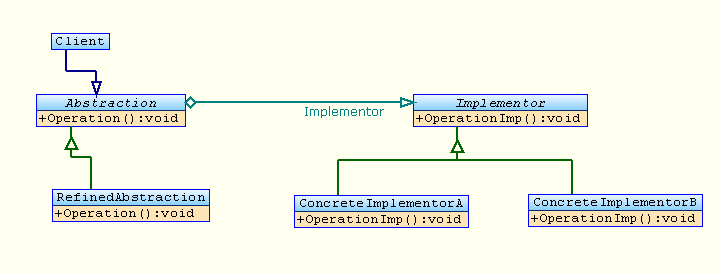
\includegraphics[scale=1]{Bridge.png} 

\title{\textbf{Anexo\\}}

Repositorio del documento en \LaTeX:

\url{https://github.com/IgnacioBriones/tarea3-ayudantia-ISW}

\end{document}